% Tiny arXiv-style preprint: basic building blocks behind the EWIGO library.
% Compiles with pdflatex (listings + literate handles the Lean unicode).
%   pdflatex ewigo-blocks.tex   (run twice for references)
\documentclass[11pt]{article}

\usepackage[utf8]{inputenc}
\usepackage[T1]{fontenc}
\usepackage[margin=1.25in]{geometry}
\usepackage{amsmath,amssymb}
\usepackage{xcolor}
\usepackage{listings}
\usepackage{tikz}
\usepackage{tikz-cd}
\usepackage{pgfplots}
\pgfplotsset{compat=1.16}
\usetikzlibrary{positioning,arrows.meta}

\usepackage{parskip}          % whitespace between paragraphs
\setlength{\parskip}{0.9em}
\linespread{1.12}

% --- a light Lean style for listings (literate maps the unicode) --------------
\definecolor{leanbg}{gray}{0.97}
\definecolor{leankw}{rgb}{0.30,0.20,0.65}
\definecolor{leancm}{rgb}{0.35,0.45,0.35}
\lstdefinestyle{lean}{
  backgroundcolor=\color{leanbg},
  basicstyle=\ttfamily\small,
  keywordstyle=\color{leankw}\bfseries,
  commentstyle=\color{leancm}\itshape,
  morekeywords={def,theorem,lemma,structure,where,fun,Prop,Finset,Type,
    univ,filter,card,instance,variable,namespace,end,open,noncomputable},
  morecomment=[l]{--},
  columns=fullflexible,
  keepspaces=true,
  showstringspaces=false,
  frame=single,
  framesep=6pt,
  xleftmargin=4pt,
  aboveskip=1.0em, belowskip=1.0em,
  literate=
    {ℕ}{{$\mathbb{N}$}}1 {ℤ}{{$\mathbb{Z}$}}1 {ℝ}{{$\mathbb{R}$}}1
    {→}{{$\rightarrow$}}1 {↦}{{$\mapsto$}}1 {∀}{{$\forall$}}1 {∃}{{$\exists$}}1
    {∑}{{$\sum$}}1 {∘}{{$\circ$}}1 {≠}{{$\neq$}}1 {≤}{{$\leq$}}1 {≥}{{$\geq$}}1
    {∧}{{$\wedge$}}1 {∨}{{$\vee$}}1 {↔}{{$\leftrightarrow$}}1 {≃}{{$\simeq$}}1
    {⊆}{{$\subseteq$}}1 {⊊}{{$\subsetneq$}}1 {×}{{$\times$}}1 {∈}{{$\in$}}1
    {·}{{$\cdot$}}1 {≅}{{$\cong$}}1 {⟨}{{$\langle$}}1 {⟩}{{$\rangle$}}1
    {₀}{{$_0$}}1 {₁}{{$_1$}}1 {₂}{{$_2$}}1 {₃}{{$_3$}}1 {₄}{{$_4$}}1
    {²}{{$^2$}}1 {³}{{$^3$}}1 {ᵈ}{{$^d$}}1 {ω}{{$\omega$}}1 {δ}{{$\delta$}}1
    {φ}{{$\varphi$}}1 {κ}{{$\kappa$}}1
}
\lstset{style=lean}
% ------------------------------------------------------------------------------

\title{\bf Small Pictures of Difference Maps\\[2pt]
  \large Basic Building Blocks, in Algebra, Geometry and Combinatorics}
\author{}
\date{}

\begin{document}
\maketitle

\begin{abstract}\noindent
This note collects the \emph{simplest} pieces behind a Lean~4 library on
difference maps over groups of exponent two.  Each piece is shown three ways:
a short formula, a small picture, and the matching Lean snippet.  Nothing here
needs deep theory --- every block already lives in Mathlib.
\end{abstract}

\bigskip

\section{The carrier: a cube}

The carrier is a finite abelian group where every element is its own inverse:
\[
  a + a = 0 \qquad\text{for all } a .
\]

Such a group is just a vector space over the two element field.  A group of size
$2^n$ is the \emph{Boolean cube} $\{0,1\}^n$, with bitwise XOR as addition.

\begin{center}
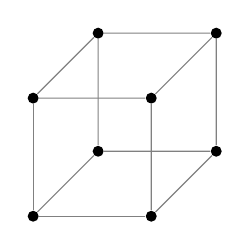
\begin{tikzpicture}[scale=1.5,every node/.style={circle,fill=black,inner sep=1.4pt}]
  \def\d{0.55}
  \node (000) at (0,0) {}; \node (100) at (1,0) {};
  \node (010) at (\d,\d) {}; \node (110) at ({1+\d},\d) {};
  \node (001) at (0,1) {}; \node (101) at (1,1) {};
  \node (011) at (\d,{1+\d}) {}; \node (111) at ({1+\d},{1+\d}) {};
  \begin{scope}[every path/.style={draw,gray}]
    \draw (000)--(100); \draw (000)--(010); \draw (000)--(001);
    \draw (100)--(110); \draw (100)--(101);
    \draw (010)--(110); \draw (010)--(011);
    \draw (001)--(101); \draw (001)--(011);
    \draw (110)--(111); \draw (101)--(111); \draw (011)--(111);
  \end{scope}
\end{tikzpicture}

{\small The group of size $2^3$: eight points, edges = flip one bit.}
\end{center}

In the library the carrier is axiomatised (no named algebra is assumed):

\begin{lstlisting}
ax_prod_comm : ∀ a b, prod_ a b = prod_ b a       -- abelian
ax_prod_unit : ∀ a, prod_ unit_ a = a             -- has a zero
ax_prod_inv  : ∀ a, prod_ (inv_ a) a = unit_      -- has inverses
ax_char2     : ∀ a, prod_ a a = unit_             -- exponent two
\end{lstlisting}

\section{Freshman's dream: a commuting square}

In characteristic two, squaring is \emph{additive}:
\[
  (a+b)^2 \;=\; a^2 + b^2 .
\]

So the squaring map $\varphi(x)=x^2$ (the Frobenius map) makes a square commute:

\begin{center}
\begin{tikzcd}[column sep=large,row sep=large]
  G\times G \arrow[r,"+"] \arrow[d,"\varphi\times\varphi"'] & G \arrow[d,"\varphi"] \\
  G\times G \arrow[r,"+"'] & G
\end{tikzcd}
\end{center}

This is already in Mathlib:

\begin{lstlisting}
-- Mathlib: in characteristic p,
add_pow_char : (a + b) ^ p = a ^ p + b ^ p
\end{lstlisting}

\section{The difference map}

Fix a direction $a$.  The difference of a map $f$ in direction $a$ is
\[
  D_a f(x) \;=\; f(x+a) - f(x) .
\]

Geometrically: slide the graph of $f$ left by $a$, then subtract.

\begin{center}
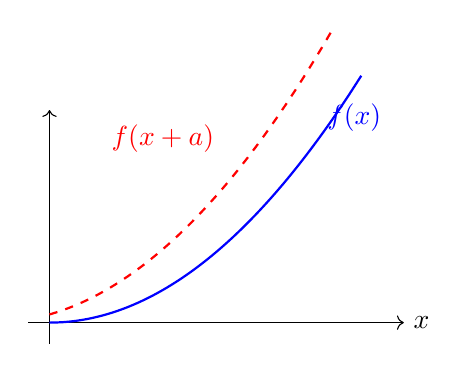
\begin{tikzpicture}[scale=0.9]
  \draw[->] (-0.3,0)--(5,0) node[right]{$x$};
  \draw[->] (0,-0.3)--(0,3) node[above]{};
  \draw[thick,blue,domain=0:4.4,smooth] plot (\x,{0.18*(\x)*(\x)});
  \draw[thick,red,dashed,domain=0:4.0,smooth] plot (\x,{0.18*(\x+0.8)*(\x+0.8)});
  \node[blue] at (4.3,2.9) {$f(x)$};
  \node[red]  at (1.6,2.6) {$f(x+a)$};
\end{tikzpicture}

{\small The dashed curve is $f(x+a)$; the difference is the gap.}
\end{center}

The library writes this for both a concrete field and an abstract carrier:

\begin{lstlisting}
def D (f : F → F) (a x : F) : F := f (x + a) - f x

def tDiff (d : ℕ) (a x : S.obj) : S.obj :=
  S.prod_ (S.endo d (S.prod_ x a)) (S.inv_ (S.endo d x))
\end{lstlisting}

\section{Fibers and width: a partition}

Fix a direction $a$ and a value $b$.  The \emph{fiber} is the set of inputs that
the difference sends to $b$, and the \emph{width} is its size:
\[
  \mathrm{fib}(a,b) = \{\, x : D_a f(x) = b \,\},
  \qquad
  \mathrm{wid}(a,b) = \bigl|\mathrm{fib}(a,b)\bigr| .
\]

As $b$ ranges over the group, the fibers tile the whole carrier:
\[
  \sum_b \mathrm{wid}(a,b) \;=\; |G| .
\]

\begin{center}
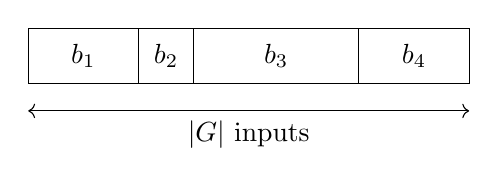
\begin{tikzpicture}[scale=0.7]
  \def\w{8}
  \draw (0,0) rectangle (\w,1);
  \foreach \x/\lab in {0/$b_1$,2/$b_2$,3/$b_3$,6/$b_4$} {
    \draw (\x,0)--(\x,1);
  }
  \node at (1,0.5){$b_1$}; \node at (2.5,0.5){$b_2$};
  \node at (4.5,0.5){$b_3$}; \node at (7,0.5){$b_4$};
  \draw[<->] (0,-0.5)--(\w,-0.5) node[midway,below]{$|G|$ inputs};
\end{tikzpicture}

{\small Each block is one fiber; the block widths add up to $|G|$.}
\end{center}

\begin{lstlisting}
def fib (d : ℕ) (a b : S.obj) : Finset S.obj :=
  univ.filter (fun x => tDiff S d a x = b)

def wid (d : ℕ) (a b : S.obj) : ℕ := (fib S d a b).card

theorem wid_partition (d : ℕ) (a : S.obj) :
    ∑ b, wid S d a b = Fintype.card S.obj
\end{lstlisting}

\section{APN: width at most two}

A map is \emph{almost perfect nonlinear} (APN) when every fiber in every nonzero
direction has size $0$ or $2$:
\[
  \mathrm{wid}(a,b) \in \{0,2\} \qquad (a\neq 0).
\]

So the \emph{width spectrum} is very flat --- only two bars:

\begin{center}
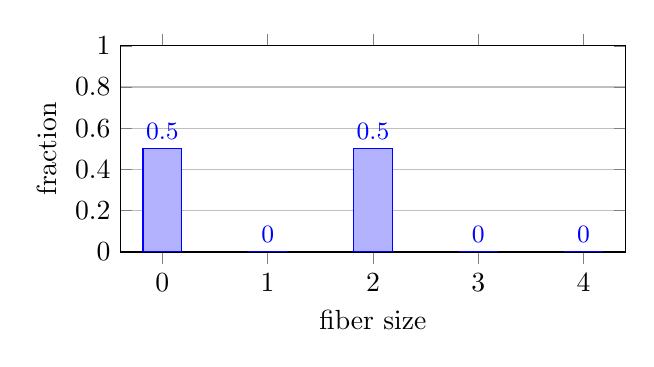
\begin{tikzpicture}
\begin{axis}[
   ybar, width=8cm, height=4.2cm,
   ymin=0, ymax=1, xtick={0,1,2,3,4},
   xlabel={fiber size}, ylabel={fraction},
   bar width=14pt, ymajorgrids,
   nodes near coords, every node near coord/.append style={font=\small},
]
\addplot coordinates {(0,0.5) (1,0) (2,0.5) (3,0) (4,0)};
\end{axis}
\end{tikzpicture}

{\small An APN map: half the values are missed, half are hit exactly twice.}
\end{center}

\begin{lstlisting}
def IsΩUniform (ω : ℕ) (f : F → F) : Prop :=
  ∀ a, a ≠ 0 → ∀ b, N f a b = 0 ∨ N f a b = ω

def IsAPN (f : F → F) : Prop := IsΩUniform 2 f
\end{lstlisting}

\section{The graph as a Sidon set}

Read the same condition in additive combinatorics.  The \emph{graph}
$\{(x,f(x))\}$ is a \emph{Sidon set}: it contains no nontrivial parallelogram,
i.e. four graph points adding to zero must already be paired up.

\begin{center}
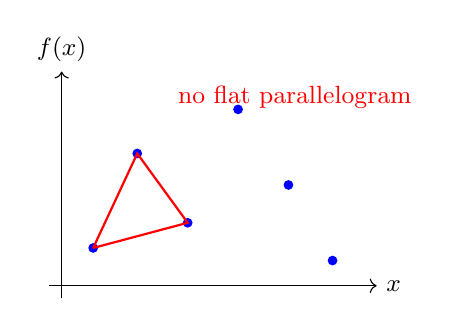
\begin{tikzpicture}[scale=0.8,every node/.style={font=\small}]
  \draw[->] (-0.2,0)--(5,0) node[right]{$x$};
  \draw[->] (0,-0.2)--(0,3.4) node[above]{$f(x)$};
  \foreach \x/\y in {0.5/0.6, 1.2/2.1, 2.0/1.0, 2.8/2.8, 3.6/1.6, 4.3/0.4}
    \fill[blue] (\x,\y) circle (2.2pt);
  % a forbidden parallelogram, crossed out
  \draw[red,thick] (0.5,0.6)--(1.2,2.1)--(2.0,1.0)--(0.5,0.6);
  \node[red] at (3.7,3.0) {no flat parallelogram};
\end{tikzpicture}
\end{center}

\begin{lstlisting}
def IsSidonGraph (f : F → F) : Prop :=
  ∀ p₁ p₂ p₃ p₄ : F × F,
    isInGraph f p₁ → isInGraph f p₂ →
    isInGraph f p₃ → isInGraph f p₄ →
    p₁ + p₂ + p₃ + p₄ = 0 →
    (p₁ = p₂ ∧ p₃ = p₄) ∨ (p₁ = p₃ ∧ p₂ = p₄) ∨ (p₁ = p₄ ∧ p₂ = p₃)
\end{lstlisting}

\section{Maps between systems: a category}

Finally, systems and the maps that respect their structure form a category.
A morphism keeps addition and commutes with the endomorphism family:

\begin{center}
\begin{tikzcd}[column sep=large,row sep=large]
  S \arrow[r,"f"] \arrow[d,"\mathrm{endo}_d"'] & T \arrow[d,"\mathrm{endo}_d"] \\
  S \arrow[r,"f"'] & T
\end{tikzcd}
\end{center}

\begin{lstlisting}
structure Mor (S T : EndoSys) where
  f    : S.obj → T.obj
  pres : ∀ a b, f (S.prod_ a b) = T.prod_ (f a) (f b)
  nat  : ∀ d x, f (S.endo d x) = T.endo d (f x)
\end{lstlisting}

Equivalence classes of such maps split into a finer level (affine, EA) sitting
inside a coarser one (CCZ):
\[
  \mathrm{EA} \;\subsetneq\; \mathrm{CCZ}.
\]

\bigskip
\begin{center}\small
Every block above is elementary; together they are the alphabet of the library.
\end{center}

\end{document}
